\documentclass[letterpaper]{article}
\usepackage{aaai2026}
\usepackage{times}
\usepackage{helvet}
\usepackage{courier}
\usepackage[hyphens]{url}
\usepackage{graphicx}
\urlstyle{rm}
\def\UrlFont{\rm}
\usepackage{natbib}
\usepackage{caption}
\frenchspacing
\setlength{\pdfpagewidth}{8.5in}
\setlength{\pdfpageheight}{11in}
\pdfinfo{
/TemplateVersion (2026.1)
}
\setcounter{secnumdepth}{2}

\usepackage{algorithm}
\usepackage{algpseudocode}
\usepackage{amsmath}
\usepackage{amssymb}
\usepackage{longtable}
\usepackage{booktabs}
\usepackage{tikz}
\usepackage[capitalize,noabbrev]{cleveref}
\usetikzlibrary{positioning, fit, backgrounds, calc, decorations.pathreplacing}

\newcommand{\method}{\texttt{cuMODD}}

% \title{Parallel Decision Diagrams-based Multiobjective Discrete Optimization} %TODO Please add
\title{Parallel Decision Diagram-based Multiobjective Discrete Optimization} %TODO Please add

% \title{\method{}: GPU-Accelerated Multiobjective Discrete Optimization using Decision Diagrams} %TODO Please add

\author{
Rahul Patel\textsuperscript{\rm 1},
Elias B. Khalil\textsuperscript{\rm 1}
}
\affiliations{
\textsuperscript{\rm 1}Department of Mechanical and Industrial Engineering, University of Toronto, Canada\\
rm.patel@mail.utoronto.ca, elias.khalil@utoronto.ca
}

\newcommand{\mink}{\oplus}

\begin{document}

\maketitle

%TODO mandatory: add short abstract of the document
\begin{abstract}
Decision diagrams (DDs) have recently emerged as a state-of-the-art technique for solving multiobjective discrete optimization problems by quickly enumerating their Pareto frontier (PF). Existing implementations rely on serial algorithms for PF enumeration, where the primary computational bottleneck arises from repeatedly performing dominance filtering at each node of the DD.
% However, dominance filtering can be parallelized to accelerate the enumeration further.
This work studies the impact of parallelizing dominance filtering on PF enumeration time. We evaluate the parallel algorithms on benchmark instances of the multiobjective knapsack, set packing, and traveling salesperson problems.
Across instance sizes, the maximum speed-up achieved by a GPU variant is $7.49\times$ for MOKP, $15.08\times$ for MOSPP, and $13.60\times$ for MOTSP relative to the state-of-the-art serial implementation.
The maximum speed-up achieved by the best parallel CPU variant is $3.36\times$ for MOKP, $2.68\times$ for MOSPP, and $5.75\times$ for MOTSP relative to the same baseline, with the caveat that it is able to solve more instances than the GPU variant.
The code is available at \url{https://anonymous.4open.science/r/PDD}.
\end{abstract}


\section{Introduction}
Multiobjective discrete optimization (MODO) \cite{ehrgott2005multicriteria,ehrgott2016exact,miettinen1999nonlinear} problems arise naturally in many applications where conflicting criteria need to be considered simultaneously in conjunction with constraints and integer variables. While problem-specific \cite{Vianna2014AMG} and generic evolutionary heuristics \cite{Deb2002AFA} have been developed for this problem class, recovering the exact Pareto frontier (PF) is desirable in critical applications such as healthcare, finance, and infrastructure planning. Over the past decade, decision diagrams (DDs) \cite{Cir2018DecisionDF} have gained traction as an effective framework for solving discrete problems that can be cast in the language of dynamic programming. As a data structure, the DD is an implicit representation of all feasible solutions to a problem. Naturally, one can enumerate the subset of such feasible solutions that are Pareto-optimal by using the multicriteria-shortest path algorithm on the network represented by a DD~\cite{garroppo2010survey}. This approach has been shown to be quite efficient in practice, yielding exact Pareto frontiers rather quickly for problems with 2-7 objectives and tens to hundreds of decision variables \cite{bergman2022network}.

Despite the success of DD-based solvers, extracting the exact Pareto frontier remains computationally demanding. The primary bottleneck lies in the state-space expansion, specifically the localized Pareto dominance filtering performed at each node to discard suboptimal labels. Because dominance checking requires pairwise comparisons among all candidate objective vectors at a node, its worst-case time complexity grows quadratically with the size of the intermediate frontiers. As the number of objectives or the size of the problem increases, this filtering step becomes the bottleneck, limiting the applicability of serial DD solvers.

Simultaneously, the proliferation of graphics processing units (GPUs) due to the rise of deep learning has prompted optimization researchers to reconsider classical algorithms and attempt to parallelize them for improved scalability \cite{ben2019demystifying}. GPUs are throughput-oriented processors designed to execute thousands of concurrent threads. The massive amount of independent, pairwise vector comparisons required during dominance filtering makes this specific bottleneck highly amenable to the \emph{Single Instruction Multiple Thread} (SIMT) architecture of GPUs.

To address this computational bottleneck, we introduce the first parallel DD-based framework for MODO. Through a careful analysis of the PF enumeration process, we identify opportunities for both node-level and candidate-level parallel computation. We propose static and dynamic resource allocation schemes that take into account the nature of the hardware being used (central processing unit (CPU) or GPU) to efficiently balance the varying workloads across the DD layers.

The main contributions of this paper are summarized as follows:
\begin{itemize}
    \item We present the first parallel algorithm for exact PF enumeration on DDs, identifying key opportunities for concurrent state expansion and dominance filtering.
    \item We design and implement novel static and dynamic memory and thread allocation schemes tailored for both multi-core CPUs and massively parallel GPUs, effectively mitigating the hazards of data races and synchronization overhead.
    \item We conduct extensive computational experiments on benchmark instances of the multiobjective knapsack, set packing, and traveling salesperson problems with up to seven objectives.
    \item We demonstrate that our parallelization schemes achieve substantial reductions in wall-clock time compared to the state-of-the-art serial enumeration baseline, achieving speedups of up to X$\times$ on CPUs and Y$\times$ on GPUs.
\end{itemize}

The remainder of this paper is organized as follows. \Cref{sec:prelim} provides the necessary background on MODO, DDs, and GPU architecture. \Cref{sec:method} details our parallel enumeration methodology and resource allocation schemes. \Cref{sec:results} presents the computational evaluation across various problem classes. The related work is provided in \Cref{sec:related}. Finally, \Cref{sec:conclusion} concludes the paper and discusses avenues for future work.

\section{Preliminaries}
\label{sec:prelim}
\subsection{Multiobjective Discrete Optimization}
\label{sec:prelim_modo}
A MODO problem can be defined as the minimization of an $m$-dimensional objective vector function $\mathbf{f}(\mathbf{x}) = (f_1(\mathbf{x}), f_2(\mathbf{x}), \dots, f_m(\mathbf{x}))^\top$ subject to $\mathbf{x} \in \mathcal{X}$. Here, $\mathbf{x} = (x_1, x_2, \dots, x_n)^\top$ represents a vector of discrete decision variables, and $\mathcal{X} \subseteq \mathbb{Z}^n$ is the bounded, discrete feasible region. We compare different feasible solutions based on the principle of \emph{Pareto dominance}. For any two feasible solutions $\mathbf{x}^1, \mathbf{x}^2 \in \mathcal{X}$, the solution $\mathbf{x}^1$ is said to Pareto dominate $\mathbf{x}^2$, denoted by $\mathbf{f}(\mathbf{x}^1) \prec \mathbf{f}(\mathbf{x}^2)$, if $f_i(\mathbf{x}^1) \le f_i(\mathbf{x}^2)$ for all $i \in \{1, \dots, m\}$, and there exists at least one index $j \in \{1, \dots, m\}$ strictly satisfying $f_j(\mathbf{x}^1) < f_j(\mathbf{x}^2)$.
An objective vector $\mathbf{y}^\star = \mathbf{f}(\mathbf{x}^\star)$ associated with a feasible solution $\mathbf{x}^\star \in \mathcal{X}$ is defined as a \emph{nondominated point} if there exists no other feasible solution $\mathbf{x} \in \mathcal{X}$ such that $\mathbf{f}(\mathbf{x}) \prec \mathbf{y}^\star$. The collection of all such nondominated points across the entire feasible region constitutes the \emph
{Pareto frontier} (or nondominated frontier) of the MODO problem. Mathematically, this frontier is expressed as $\mathcal{Y}_N = \{\mathbf{f}(\mathbf{x}) \mid \mathbf{x} \in \mathcal{X}, \nexists \, \mathbf{x}' \in \mathcal{X} \text{ such that } \mathbf{f}(\mathbf{x}') \prec \mathbf{f}(\mathbf{x})\}$. The fundamental aim in exact multiobjective optimization is to completely enumerate this Pareto frontier, providing decision-makers with the exact trade-offs among the competing criteria.


\subsection{Decision Diagrams for Multiobjective Discrete Optimization}
\label{sec:prelim_dd}


A DD is a directed layered acyclic graph $\mathcal{D} = (\mathcal{N}, \mathcal{A})$ defined by a node set $\mathcal{N}$ and an arc set $\mathcal{A}$. The node set is partitioned into $n+1$ strictly sequential layers, $\mathcal{N} = \mathcal{L}_1 \cup \dots \cup \mathcal{L}_{n+1}$, corresponding to the sequence of the $n$ decision variables. The first layer $\mathcal{L}_1$ contains only the \emph{root node} $\mathbf{r}$, and the final layer $\mathcal{L}_{n+1}$ contains only the \emph{terminal node} $\mathbf{t}$.

The arcs in $\mathcal{A}$ are directed from nodes in layer $\mathcal{L}_j$ to nodes in layer $\mathcal{L}_{j+1}$ for $j \in \{1, \dots, n\}$. Every arc $a \in \mathcal{A}$ originating from layer $\mathcal{L}_j$ possesses two key attributes: an \emph{assignment value} $d(a) \in \mathbb{Z}$, which dictates the value assigned to the decision variable $x_j$, and an \emph{objective weight} $\mathbf{v}(a) \in \mathbb{R}^m$, which represents the transition's contribution to the $m$-dimensional objective function. A path $p = (a_1, \dots, a_n)$ from the root $\mathbf{r}$ to the terminal node $\mathbf{t}$ encodes a complete decision vector $\mathbf{x}(p) = (d(a_1), \dots, d(a_n))^\top \in \mathbb{Z}^n$, with an associated objective vector obtained by accumulating the arc weights along the path $\mathbf{v}(p) = \sum_{i=1}^n \mathbf{v}(a_i)$.


Let $\mathcal{X}_{\mathcal{D}} = \{ \mathbf{x}(p) \mid p \text{ is an } \mathbf{r}-\mathbf{t} \text{ path in } \mathcal{D} \}$ denote the set of solutions encoded by the diagram. A DD is said to be \emph{exact} for a given problem if it represents the feasible region ($\mathcal{X}_{\mathcal{D}} = \mathcal{X}$) and the path evaluations correctly compute the objective function ($\mathbf{v}(p) = \mathbf{f}(\mathbf{x}(p))$ for all paths). In this case, the image of the encoded solutions in the objective space is $\mathcal{Y}_{\mathcal{D}} = \{ \mathbf{v}(p) \mid p \text{ is an } \mathbf{r}\text{-to-}\mathbf{t} \text{ path} \}$. The nondominated vectors extracted from $\mathcal{Y}_{\mathcal{D}}$ constitute the exact Pareto frontier $\mathcal{Y}_N$ of the original MODO problem.

\begin{algorithm}[tbp!]
\caption{Coupled Pareto Frontier Enumeration}
\label{alg:coupled_pf}
\begin{algorithmic}[1]
\Require Exact decision diagram $\mathcal{D} = (\mathcal{N}, \mathcal{A})$ with layers $\mathcal{L}_1, \dots, \mathcal{L}_{n+1}$
\Procedure{FilterDominated}{$\mathcal{Y}$} \Comment{$\mathcal{O}(|\mathcal{Y}|^2)$}
    \State \Return $\mathcal{Y} \gets \{ \mathbf{y} \in \mathcal{Y} \mid \nexists \, \mathbf{y}' \in \mathcal{Y} \text{ such that } \mathbf{y}' \prec \mathbf{y} \}$
\EndProcedure
\Procedure{ExpandTopDown}{$j, \mathcal{Y}^{\downarrow}$}
    \For{\textbf{each} node $u \in \mathcal{L}_j$}
        \For{\textbf{each} arc $a = (u, v)$ originating from $u$}
            \State $\mathcal{Y}^{\downarrow}(v) \gets \mathcal{Y}^{\downarrow}(v) \cup (\mathcal{Y}^{\downarrow}(u) \oplus \{\mathbf{v}(a)\})$
            \State $\mathcal{Y}^{\downarrow}(v) \gets$ \Call{FilterDominated}{$\mathcal{Y}^{\downarrow}(v)$}
        \EndFor
    \EndFor
    \State \Return $\mathcal{Y}^{\downarrow}$
\EndProcedure
\Procedure{ExpandBottomUp}{$j, \mathcal{Y}^{\uparrow}$}
    \For{\textbf{each} node $v \in \mathcal{L}_j$}
        \For{\textbf{each} arc $a = (u, v)$ entering $v$ from $u \in \mathcal{L}_{j-1}$}
            \State $\mathcal{Y}^{\uparrow}(u) \gets \mathcal{Y}^{\uparrow}(u) \cup (\mathcal{Y}^{\uparrow}(v) \oplus \{\mathbf{v}(a)\})$
            \State $\mathcal{Y}^{\uparrow}(u) \gets$ \Call{FilterDominated}{$\mathcal{Y}^{\uparrow}(u)$}
        \EndFor
    \EndFor
    \State \Return $\mathcal{Y}^{\uparrow}$
\EndProcedure

\State $\mathcal{Y}^{\downarrow}(u) \gets \emptyset$, $\mathcal{Y}^{\uparrow}(u) \gets \emptyset$ for all $u \in \mathcal{N}$
\State $\mathcal{Y}^{\downarrow}(\mathbf{r}) \gets \{\mathbf{0}\}, \mathcal{Y}^{\uparrow}(\mathbf{t}) \gets \{\mathbf{0}\}$ \Comment{$\mathbf{r}$ is root, $\mathbf{t}$ is terminal}
\State $i_{\text{td}} \gets 1$, $i_{\text{bu}} \gets n+1$
\While{$i_{\text{td}} \neq i_{\text{bu}}$}
    \State Dynamically decide whether to expand top-down or bottom-up
    \If{expanding top-down}
        \State \Call{ExpandTopDown}{$i_{\text{td}}, \mathcal{Y}^{\downarrow}$}, $i_{\text{td}} \gets i_{\text{td}} + 1$
    \Else
        \State \Call{ExpandBottomUp}{$i_{\text{bu}}, \mathcal{Y}^{\uparrow}$}, $i_{\text{bu}} \gets i_{\text{bu}} - 1$
    \EndIf
\EndWhile
\State $c \gets i_{\text{td}}, \mathcal{Y}_N \gets \emptyset$
\For{\textbf{each} node $u \in \mathcal{L}_c$}
    \State $\mathcal{Y}(u) \gets \mathcal{Y}^{\downarrow}(u) \oplus \mathcal{Y}^{\uparrow}(u)$ \Comment{$\mathcal{O}(|\mathcal{Y}^{\downarrow}(u)||\mathcal{Y}^{\uparrow}(u)|)$}
\EndFor
\For{\textbf{each} node $u \in \mathcal{L}_c$}
    \State $\mathcal{Y}_N \gets$ \Call{FilterDominated}{$\mathcal{Y}_N \cup \mathcal{Y}(u)$}
\EndFor
\State \Return $\mathcal{Y}_N$
\end{algorithmic}
\end{algorithm}

To extract this exact Pareto frontier $\mathcal{Y}_N$ from an exact decision diagram $\mathcal{D}$, we can employ the \emph{coupled enumeration scheme}, which dynamically interleaves top-down and bottom-up layer expansion, as detailed in \Cref{alg:coupled_pf}. This dynamic layer cutset methodology mitigates intermediate label explosion. Initially, a top-down layer pointer $i_{\text{td}}$ is set to layer 1 and a bottom-up pointer $i_{\text{bu}}$ is set to layer $n+1$. At each step, the scheme dynamically decides whether to expand the top-down frontier $\mathcal{Y}^{\downarrow}$ to layer $i_{\text{td}}+1$ or the bottom-up frontier $\mathcal{Y}^{\uparrow}$ to layer $i_{\text{bu}}-1$. This process continues until the two frontiers meet at a \emph{cutset} layer $c$ (i.e., $i_{\text{td}} = i_{\text{bu}}$). Finally, for each node $u \in \mathcal{L}_c$, the algorithm computes the convolution of its top-down and bottom-up labels (\Cref{alg:coupled_pf}, line 35), taking the pairwise sum of these vectors. The merging of these combined sets and the repeated application of a dominance filter produce the exact Pareto frontier $\mathcal{Y}_N$.

% To maintain efficiency and prevent exponential growth of these label sets, a localized Pareto dominance filtering is performed at each node after a layer expansion (e.g. \Cref{alg:coupled_pf}, line 7 and 17). This localized filtering removes any vectors that are Pareto dominated by other vectors within the same set, ensuring that only nondominated partial paths are propagated forward. The dominance filtering operation requires pairwise comparisons among vectors in $\mathcal{Y}^{\downarrow}(v)$ and has worst-case complexity $\mathcal{O}(|\mathcal{Y}^{\downarrow}(v)|^2)$. This step is the key bottleneck in enumeration and consumes the most time.
A special case of the coupled enumeration scheme is the \emph{top-down enumeration scheme}, in which the bottom-up layer pointer $i_{\text{bu}}$ is fixed to the layer $n+1$. As such, only operations involving `ExpandTopDown` are executed, and the cutset layer naturally occurs at $c = n+1$. In this case, upon completion of the final layer processing, the label set $\mathcal{Y}^{\downarrow}(\mathbf{t})$ at the terminal node directly corresponds to the exact Pareto frontier $\mathcal{Y}_N$. This approach is outlined in Algorithm~\ref{alg:top_down_pf}. Note that we did not perform convolution or repeated dominance filtering (\Cref{alg:coupled_pf}, lines 33 to 37) in this approach.

\begin{algorithm}[htbp]
\caption{Top-Down Pareto Frontier Enumeration}
\label{alg:top_down_pf}
\begin{algorithmic}[1]
\Require Exact decision diagram $\mathcal{D} = (\mathcal{N}, \mathcal{A})$ with layers $\mathcal{L}_1, \dots, \mathcal{L}_{n+1}$
\State $\mathcal{Y}^{\downarrow}(u) \gets \emptyset$ for all $u \in \mathcal{N}$
\State $\mathcal{Y}^{\downarrow}(\mathbf{r}) \gets \{\mathbf{0}\}$ \Comment{$\mathbf{r}$ is the root node in $\mathcal{L}_1$, $\mathbf{0} \in \mathbb{R}^m$}
\For{$j = 1$ \textbf{to} $n$}
    \State \Call{ExpandTopDown}{$j, \mathcal{Y}^{\downarrow}$}
\EndFor
\State \Return $\mathcal{Y}^{\downarrow}(\mathbf{t})$ \Comment{$\mathbf{t}$ is the terminal node in $\mathcal{L}_{n+1}$}
\end{algorithmic}
\end{algorithm}


\subsection{Graphics Processing Unit}
\label{sec:prelim_gpu}

GPUs are throughput-oriented processors that achieve high performance by executing many lightweight threads in parallel. In contrast, CPUs comprise a small number of complex cores optimized for low-latency execution and sophisticated control flow. This architectural difference makes GPUs particularly effective for data-parallel workloads in which the same operation is applied independently across many inputs \cite{lindholm2008nvidia}.
\Cref{fig:gpu_arch} illustrates the GPU execution and memory hierarchy. Computation is launched as a \emph{kernel}, which executes as a large collection of \emph{threads}. Threads are grouped into \emph{thread blocks}, and all blocks in a kernel launch form a \emph{grid} \cite{nickolls2008scalable}. The GPU schedules thread blocks onto \emph{Streaming Multiprocessors} (SMs), where each SM can host multiple blocks concurrently and executes threads in a \emph{Single Instruction Multiple Thread} (SIMT) manner, where threads follow the same instruction stream while operating on different data.


\begin{figure}[tbp]
    \centering
    \resizebox{0.5\linewidth}{!}{
    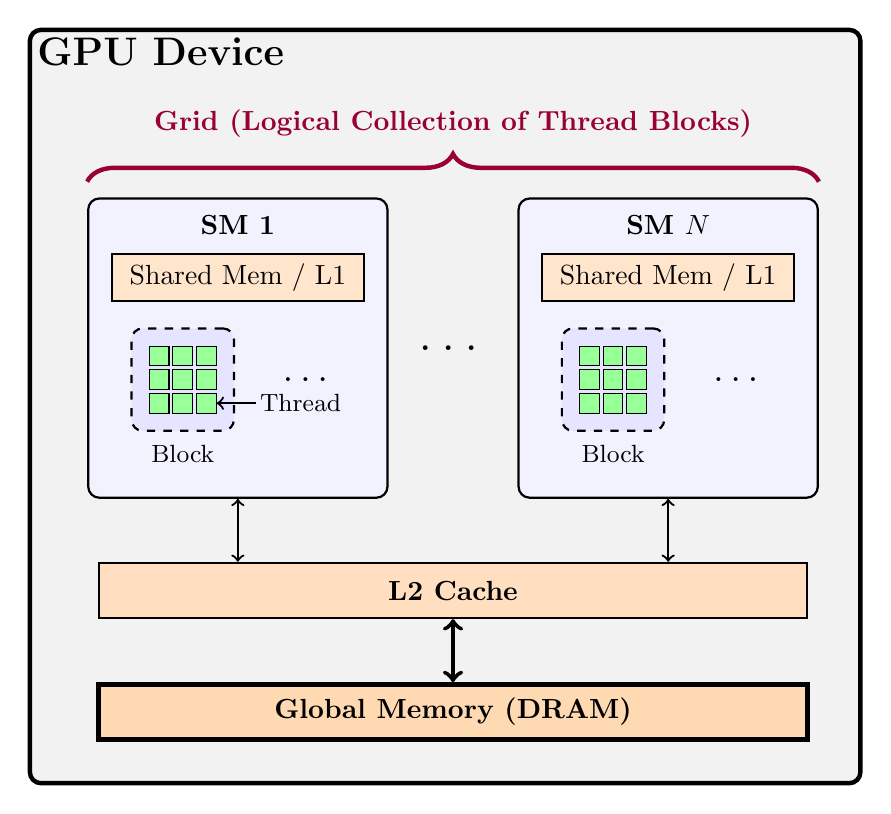
\begin{tikzpicture}[
        sm/.style={draw, thick, fill=blue!5, rounded corners, minimum width=3.8cm, minimum height=3.8cm},
        block/.style={draw, dashed, thick, fill=blue!10, rounded corners, inner sep=3pt},
        thread/.style={draw, fill=green!40, minimum width=0.25cm, minimum height=0.25cm, inner sep=0pt},
        mem/.style={draw, thick, fill=orange!20, minimum width=3.2cm, minimum height=0.6cm, align=center},
        l2/.style={draw, thick, fill=orange!25, minimum width=9cm, minimum height=0.7cm, align=center},
        gmem/.style={draw, ultra thick, fill=orange!30, minimum width=9cm, minimum height=0.7cm, align=center},
        device/.style={draw, ultra thick, fill=gray!10, rounded corners, inner sep=15pt}
    ]

    % SM 1
    \node[sm] (sm1) at (0,0) {};
    \node[anchor=north, font=\bfseries, yshift=-0.1cm] at (sm1.north) {SM 1};
    \node[mem, anchor=north, yshift=-0.7cm] (smem1) at (sm1.north) {Shared Mem / L1};

    % SM 1 - Block 1
    \node[block, minimum width=1.3cm, minimum height=1.3cm] (s1b1) at ($(sm1.center) + (-0.7, -0.4)$) {};
    \node[font=\small, anchor=north, yshift=-0.05cm] at (s1b1.south) {Block};
    \foreach \i/\x in {1/-0.3, 2/0, 3/0.3} {
        \foreach \j/\y in {1/0.3, 2/0, 3/-0.3} {
            \node[thread] (s1b1t\i\j) at ($(s1b1.center) + (\x, \y)$) {};
        }
    }

    % SM 1 - Multiple Blocks Dots
    \node[font=\Large] at ($(sm1.center) + (0.9, -0.4)$) {\dots};

    % Explicit annotation for Threads
    \draw[<-, thick] (s1b1t33.east) -- ++(0.5, 0) node[right, font=\small, inner sep=1pt] {Thread};

    % Dots indicating more SMs
    \node[right=0.25cm of sm1, font=\huge] (dots) {\dots};

    % SM N
    \node[sm, right=0.25cm of dots] (smn) {};
    \node[anchor=north, font=\bfseries, yshift=-0.1cm] at (smn.north) {SM $N$};
    \node[mem, anchor=north, yshift=-0.7cm] (smemn) at (smn.north) {Shared Mem / L1};

    % SM N - Block 1
    \node[block, minimum width=1.3cm, minimum height=1.3cm] (snb1) at ($(smn.center) + (-0.7, -0.4)$) {};
    \node[font=\small, anchor=north, yshift=-0.05cm] at (snb1.south) {Block};
    \foreach \i/\x in {1/-0.3, 2/0, 3/0.3} {
        \foreach \j/\y in {1/0.3, 2/0, 3/-0.3} {
            \node[thread] (snb1t\i\j) at ($(snb1.center) + (\x, \y)$) {};
        }
    }

    % SM N - Multiple Blocks Dots
    \node[font=\Large] at ($(smn.center) + (0.9, -0.4)$) {\dots};

    % Logical Grid Brace
    \draw[decorate, decoration={brace, amplitude=10pt}, ultra thick, purple!80!black]
        ([yshift=0.2cm]sm1.north west) -- ([yshift=0.2cm]smn.north east)
        node[midway, above=12pt, font=\bfseries, purple!80!black] {Grid (Logical Collection of Thread Blocks)};

    % L2 Cache (Centered between SM1 and SMN)
    \node[l2, anchor=north] (l2cache) at ($(sm1.south)!0.5!(smn.south) + (0, -0.8cm)$) {\textbf{L2 Cache}};

    % Global Memory
    \node[gmem, below=0.8cm of l2cache] (globalmem) {\textbf{Global Memory (DRAM)}};

    % Connections
    \draw[<->, thick] (sm1.south) -- (sm1.south |- l2cache.north);
    \draw[<->, thick] (smn.south) -- (smn.south |- l2cache.north);
    \draw[<->, ultra thick] (l2cache.south) -- (globalmem.north);

    % Device Background Layer
    \begin{scope}[on background layer]
        % Add a hidden coordinate to push the top border up slightly for the label and brace
        \coordinate (topleft) at ([xshift=-0.2cm, yshift=1.6cm]sm1.north west);
        \node[device, fit=(topleft) (smn) (globalmem)] (gpu) {};
        \node[anchor=north west, font=\Large\bfseries] at (gpu.north west) {GPU Device};
    \end{scope}

    \end{tikzpicture}}
    \caption{Schematic representation of a GPU architecture.}
    \label{fig:gpu_arch}
\end{figure}
The memory system is also hierarchical. Threads within an SM have access to fast on-chip storage, including registers and shared memory, which enables efficient intra-block cooperation and synchronization. SMs connect to a larger, device-wide cache (L2) and ultimately to high-capacity but high-latency global memory (DRAM). Effective GPU implementations therefore aim to expose ample parallelism while limiting expensive global-memory traffic \cite{nickolls2010gpu}.
This execution model is well suited for workloads dominated by large numbers of independent arithmetic operations and comparisons. In particular, pairwise dominance checks required during PF enumeration in Algorithm~\ref{alg:top_down_pf} are natural candidates for GPU acceleration.



\section{Parallel Decision Diagram-based Pareto Frontier Enumeration}
\label{sec:method}

This section describes the methodology for leveraging parallelism during the PF enumeration. The different parallelization schemes are introduced in \Cref{sec:parallel_schemes} and their implementation details are provided in \Cref{sec:parallel_impl}.

\subsection{Parallelization Schemes}
\label{sec:parallel_schemes}

\subsubsection{Single thread per node}
In this scheme, we exploit the inherent independence of nodes within the same layer to achieve parallelism. Specifically, the processing of any node $v \in \mathcal{L}_{j+1}$ relies exclusively on the finalized objective vectors of its predecessor nodes $u \in \mathcal{L}_j$. Because the operations performed on different destination nodes do not mutate or conflict with one another's memory space, we can process multiple nodes concurrently by assigning a single, dedicated execution thread to each node.

For instance, in the coupled enumeration scheme (Algorithm~\ref{alg:coupled_pf}), the execution of \textsc{ExpandTopDown} (lines 5-10) and \textsc{ExpandBottomUp} (lines 14-19) can be parallelized over the outer loop of destination nodes.
Furthermore, at the cutset layer $\mathcal{L}_c$, the convolution of the top-down and bottom-up frontiers (lines 34-36) can be parallelized across individual nodes since each convolution operates strictly on local label sets $\mathcal{Y}^{\downarrow}(u)$ and $\mathcal{Y}^{\uparrow}(u)$ associated with node $u$.
By mapping a single thread per node, this scheme circumvents data races without the need for expensive thread synchronization mechanisms like locks.

\subsubsection{Multiple threads per node}
While assigning a single thread per node is straightforward, the overall enumeration can be further accelerated by utilizing multiple threads to process a single node collaboratively. However, a naive implementation of such a scheme presents significant synchronization hazards.
Consider the \textsc{ExpandTopDown} procedure, where multiple incoming arcs $(u,v)$ contribute to the same destination node $v$. A simplistic approach to multi-threading this step would be to assign a separate thread to each incoming arc. Each thread would expand the labels of the parent node of its assigned arc and attempt to merge and filter the generated candidates directly into the destination node's shared set, $\mathcal{Y}^{\downarrow}(v)$. This introduces the following critical synchronization issues.
\begin{enumerate}
\item \textbf{Data Races and Loss:} If threads attempt to update the shared label set concurrently without locks, memory corruption will occur, leading to the unpredictable loss of valid Pareto-optimal candidates.
\item \textbf{Synchronization Bottlenecks:} If a lock is applied to the shared label set $\mathcal{Y}^{\downarrow}(v)$ to prevent data races, the execution essentially serializes, negating the benefits of multi-threading.
\end{enumerate}
To effectively leverage multiple cores per node without succumbing to locking bottlenecks, we can trade off memory for execution speed. Rather than merging candidates into a single shared set on the fly, we can decouple the expansion phase from the filtering phase. First, threads can safely evaluate the addition for all arcs in parallel, scattering the resulting candidate labels into disjoint, pre-allocated memory segments. Once all candidates for the node are materialized in memory, a pool of threads can cooperatively perform the computationally dominant $\mathcal{O}(|\mathcal{Y}|^2)$ dominance filtering operation over this complete set of candidates, allowing multiple threads to actively prune suboptimal vectors simultaneously without locks.

Furthermore, assigning a \textit{fixed} number of threads to collaboratively process each node is suboptimal if the size of the intermediate Pareto frontiers $\mathcal{Y}^{\downarrow}(v)$ varies drastically across nodes within a given layer. If a static number of threads are allocated per node, the nodes with massive sets of incoming candidates will still bottleneck the overall layer progression, while the thread groups assigned to nodes with few candidates will prematurely finish and sit idle. Thus, an optimal multi-threaded strategy must dynamically allocate a variable number of threads to each node proportional to the size of its candidate label set to ensure an evenly balanced workload.
In practice, our CPU implementation realizes the \textit{single thread per node} scheme, while the GPU architecture allows us to efficiently realize the \textit{multiple threads per node} scheme.


\subsection{Implementation}
\label{sec:parallel_impl}


\subsubsection{Central Processing Unit}


The CPU implementation directly realizes the single thread per node parallelization scheme. At each layer $j$, the loop over destination nodes $v \in \mathcal{L}_{j+1}$ is parallelized with a \emph{dynamic work-stealing} schedule: since the number of incoming candidate labels per node varies widely across a layer, a static round-robin assignment would leave many cores idle while others process large frontier sets. Each assigned core processes all incoming arcs $(u,v)$ for its node sequentially, accumulating the Minkowski sums $\mathcal{Y}^{\downarrow}(u) \oplus \{\mathbf{v}(a)\}$ and applying the $\mathcal{O}(|\mathcal{Y}|^2)$ dominance filter entirely in thread-local memory, requiring no locks or synchronization. However, a core assigned to a node with a very large local frontier cannot offload work to idle cores, throttling the entire layer's throughput. This load-imbalance limitation motivates the GPU design below.





\subsubsection{Graphics Processing Unit}
The GPU is well-suited to realize the multiple threads per node scheme: its massively parallel architecture executes thousands of lightweight threads concurrently, making it ideal for absorbing the data-parallelism in candidate generation and dominance filtering. \Cref{alg:gpu_top_down_pf} presents the GPU-accelerated top-down enumeration, which decomposes each layer's processing into four data-parallel GPU passes that call the subroutines in Algorithms~\ref{alg:compute_arc_offsets}--\ref{alg:compact_survivors}.

\begin{algorithm}[tbp!]
\caption{GPU-Accelerated Top-Down Pareto Frontier Enumeration}
\label{alg:gpu_top_down_pf}
\begin{algorithmic}[1]
\Require DD $\mathcal{D}$ with layers $\mathcal{L}_1,\dots,\mathcal{L}_{n+1}$
\State \textbf{on CPU}: For every arc $a \in \mathcal{A}$, pack source-node index $b(a)$ and weight vector $\mathbf{v}(a)$ into flat arrays; for every node $v$, pack the incoming-arc offset array $\phi^a_v$; transfer all to GPU \Comment{One-time}
\State \textbf{on CPU}: Initialize $\mathcal{Y}^{\downarrow}(\mathbf{r}) \gets \{\mathbf{0}\}$ in GPU memory
\For{$j = 1$ \textbf{to} $n$ \textbf{[CPU outer loop]}}
    \State $\kappa, \phi^c, \Gamma \gets$ \Call{ComputeArcOffsets}{$\mathcal{Y}^{\downarrow}, b, \phi^a$}
    \State $\beta \gets$ \Call{ExpandCandidates}{$\mathcal{Y}^{\downarrow}, b, \mathbf{v}, \phi^c, \kappa$}
    \State $\sigma \gets$ \Call{FilterDominated}{$\beta, \Gamma$}
    \State $\mathcal{Y}^{\downarrow} \gets$ \Call{CompactSurvivors}{$\beta, \sigma$}
    \State Swap buffer pointers (no data copy)
\EndFor
\State \textbf{on CPU}: Copy $\mathcal{Y}^{\downarrow}(\mathbf{t})$ from GPU to host; \Return $\mathcal{Y}^{\downarrow}(\mathbf{t})$
\end{algorithmic}
\end{algorithm}
\footnotetext{For problems with tractable state-space structure (e.g., knapsack), a problem-specific dominance filter is additionally applied on the GPU after this step.}

Before entering the layer loop, the CPU serializes the DD's arc connectivity into contiguous flat arrays---the source-node index $b(a)$, the $m$-dimensional weight vector $\mathbf{v}(a)$ for every arc $a$, and the per-node incoming-arc offset array $\phi^a_v$---and transfers them to GPU global memory once (line~1), amortizing the packing cost across all layers. The outer loop executes on the CPU because each layer depends on the previous layer's filtered results. Within each layer, four GPU passes are executed.

\textbf{(1)~Arc-level offset computation} (\Cref{alg:compute_arc_offsets}): for each arc $a = (u,v)$, one GPU thread reads the source node's frontier size $|\mathcal{Y}^{\downarrow}(u)|$, yielding a per-arc candidate count $\kappa_a$. An exclusive prefix sum over these counts produces per-arc buffer offsets $\phi^c_a$, which determine where each arc's candidates will be written in the flat buffer $\beta$. The per-destination-node candidate total $\Gamma_v$ is derived from the difference between the edge offsets of the last and first incoming arcs of $v$.

\begin{algorithm}[tbp]
\caption{GPU Subroutine: Compute Arc Offsets}
\label{alg:compute_arc_offsets}
\begin{algorithmic}[1]
\Require Frontier $\mathcal{Y}^{\downarrow}$; source-node array $b[]$; incoming-arc offsets $\phi^a[]$
\Procedure{ComputeArcOffsets}{$\mathcal{Y}^{\downarrow}, b, \phi^a$}
\State $M \gets |\mathcal{A}_{\mathcal{L}_j}|$ \Comment{Number of arcs in layer $j$}
\ForAll{arcs $a = 0$ \textbf{to} $M-1$ \textbf{in parallel on GPU}} \Comment{One thread per arc}
    \State $\kappa_a \gets |\mathcal{Y}^{\downarrow}(b(a))|$
\EndFor
\State $\phi^c_0 \gets 0$
\For{$a = 1$ \textbf{to} $M$ \textbf{in parallel on GPU}}
    \State $\phi^c_a \gets \phi^c_{a-1} + \kappa_{a-1}$
\EndFor
\ForAll{nodes $v \in \mathcal{L}_{j+1}$ \textbf{in parallel on GPU}}
    \State $a_{\text{first}} \gets \phi^a_v$
    \State $a_{\text{last}} \gets \phi^a_{v{+}1}$
    \State $\Gamma_v \gets \phi^c_{a_{\text{last}}} - \phi^c_{a_{\text{first}}}$
\EndFor
\State \Return $\kappa, \phi^c, \Gamma$
\EndProcedure
\end{algorithmic}
\end{algorithm}

\textbf{(2)~Candidate expansion} (\Cref{alg:expand_candidates}): the flat buffer $\beta$ is populated with shifted labels. Each arc $a$ is assigned to a \emph{warp}---a fixed group of 32 GPU threads that execute the same instruction simultaneously, each on different data. The threads within a warp cooperatively iterate over the source node's labels, with each thread handling one label at a time. Since the prefix sum in Step~1 guarantees that each arc's output segment $[\phi^c_a,\ \phi^c_a + \kappa_a)$ is non-overlapping, threads for different arcs write to disjoint memory regions without synchronization.

\begin{algorithm}[tbp]
\caption{GPU Subroutine: Expand Candidates into Flat Buffer}
\label{alg:expand_candidates}
\begin{algorithmic}[1]
\Require Frontier $\mathcal{Y}^{\downarrow}$; source array $b[]$; arc weights $\mathbf{v}(\cdot)$; offsets $\phi^c[]$; counts $\kappa[]$
\Procedure{ExpandCandidates}{$\mathcal{Y}^{\downarrow}, b, \mathbf{v}, \phi^c, \kappa$}
\State Allocate flat buffer $\beta$ of size $\sum_a \kappa_a$
\ForAll{arcs $a$ \textbf{in parallel on GPU}}
    \State //~One warp (32 threads) per arc
    \ForAll{$k = 0, 1, \dots, \kappa_a{-}1$ \textbf{distributed across warp threads}}
        \State $\beta[\,\phi^c_a + k\,] \gets \mathcal{Y}^{\downarrow}(b(a))[k] + \mathbf{v}(a)$
    \EndFor
\EndFor
\State \Return $\beta$
\EndProcedure
\end{algorithmic}
\end{algorithm}

\textbf{(3)~Load-balanced dominance filtering} (\Cref{alg:dynamic_1D_kernel}): each destination node $v$ receives $K_v = \lceil \Gamma_v / B \rceil$ thread blocks (where $B$ is the block size). A prefix sum over $K_v$ yields a block-offset array $\phi^k$ that maps each block to its target node. A tightly packed grid of $\sum_v K_v$ blocks is launched; each block locates its target node via binary search, ensuring no blocks sit idle.

\begin{algorithm}[tbp]
\caption{GPU Dominance Filtering: Dynamic 1D Load-Balanced Scheduling}
\label{alg:dynamic_1D_kernel}
\begin{algorithmic}[1]
\Require Flat candidate buffer $\beta$; per-node candidate counts $\Gamma[]$; block size $B$
\Procedure{FilterDominated}{$\beta, \Gamma$}
\State $K[v] \gets \lceil \Gamma[v] / B \rceil$ for all $v$
% \Comment{Blocks needed per node}
\State $\phi^k_0 \gets 0$
\For{$v = 1$ \textbf{to} $|\mathcal{L}_{j+1}|$ \textbf{in parallel on GPU}}
    \State $\phi^k_v \gets \phi^k_{v-1} + K[v-1]$
\EndFor
\State $\sigma_i \gets 1$ for all candidates $i$
\ForAll{thread blocks $q = 0, \dots, \sum_v K[v] - 1$ \textbf{in parallel on GPU}}
    \State Binary search $\phi^k$ to find node $v$ s.t.\ $\phi^k_v \le q < \phi^k_{v{+}1}$
    \State $\tau \gets q - \phi^k_v$ \Comment{Tile index within node $v$}
    \State $[b,\, e) \gets$ candidate range of node $v$ in $\beta$
    \State $i \gets b + \tau \cdot B + \text{thread index within block}$
    \State \textbf{Load} $\mathbf{y}_i \gets \beta[i]$ into per-thread register (if $i < e$) \Comment{Reused across tiles}
    \State $\mathit{dominated} \gets \mathbf{false}$
    \For{tile start $s = b$ \textbf{to} $e{-}1$, \textbf{step} $B$}
        \State \textbf{Barrier}: wait for all threads in block
        \State Each thread $k$ loads $\beta[s{+}k]$ into \textbf{shared memory} slot $k$ \;(if $s{+}k < e$)
        \State \textbf{Barrier}: ensure tile is fully visible
        \If{$i < e$ \textbf{and not} $\mathit{dominated}$}
            \For{$j = 0$ \textbf{to} $\min(B,\, e{-}s){-}1$, \textbf{skip} $j = i{-}b{-}\tau B$}
                \If{shared[$j$] $\prec \mathbf{y}_i$}\; $\mathit{dominated} \gets \mathbf{true}$; \textbf{break} \EndIf
            \EndFor \Comment{Early exit within tile}
        \EndIf
        \If{$\mathit{dominated}$} \textbf{break} \EndIf \Comment{Early exit across tiles}
    \EndFor
    \If{$i < e$ \textbf{and} $\mathit{dominated}$}\; $\sigma_i \gets 0$ \EndIf
\EndFor
\State \Return $\sigma$
\EndProcedure
\end{algorithmic}
\end{algorithm}

Within each thread block, two levels of the memory hierarchy are exploited. Each thread loads its own candidate $\mathbf{y}_i$ from global GPU memory (high-latency DRAM) once into a \emph{per-thread private register} (line~10), retaining it for all tile comparisons without re-reading global memory. The $B$ block members then cooperatively load a tile of $B$ reference candidates into \emph{shared memory} (fast on-chip scratchpad visible to all threads in the block), one reference per thread (lines~13--14). Two barrier synchronizations bracket this load so all threads see a consistent tile. Each thread checks $\mathbf{y}_i$ against all $B$ references; a dominance detection immediately breaks both the within-tile and across-tile loops (lines~17--19), avoiding redundant comparisons.

\textbf{(4)~Survivor compaction} (\Cref{alg:compact_survivors}): the dominance filter produces a binary flag $\sigma_i \in \{0, 1\}$ for each candidate $i$, where $\sigma_i = 1$ indicates that candidate $i$ was not Pareto dominated. An exclusive prefix sum over these flags computes each survivor's compacted output position $\rho_i$. A final scatter pass writes only the survivors into the per-node label sets $\mathcal{Y}^{\downarrow}(v)$.

\begin{algorithm}[tbp]
\caption{GPU Subroutine: Compact Survivors}
\label{alg:compact_survivors}
\begin{algorithmic}[1]
\Require Candidate buffer $\beta$ of size $S$; binary survivor flags $\sigma[]$
\Procedure{CompactSurvivors}{$\beta, \sigma$}
\State $\rho_0 \gets 0$
\For{$i = 1$ \textbf{to} $S$} \Comment{Parallel prefix sum on GPU}
    \State $\rho_i \gets \rho_{i-1} + \sigma_{i-1}$
\EndFor
\ForAll{candidates $i = 0$ \textbf{to} $S-1$ \textbf{in parallel on GPU}} \Comment{One thread per candidate}
    \If{$\sigma_i = 1$}
        \State $\mathcal{Y}^{\downarrow}(v)[\,\rho_i\,] \gets \beta[i]$ \Comment{$v$: destination node of $i$}
    \EndIf
\EndFor
\State \Return $\mathcal{Y}^{\downarrow}$
\EndProcedure
\end{algorithmic}
\end{algorithm}

\subsubsection{GPU-Accelerated Coupled Enumeration}
While top-down expansion is highly parallel, memory consumption can scale rapidly for intermediate layers with large widths. The coupled enumeration scheme (\Cref{alg:coupled_pf}) mitigates this by dynamically progressing from both directions to meet at a cutset layer $\mathcal{L}_c$.

\Cref{alg:gpu_coupled_pf} presents the GPU-accelerated coupled enumeration orchestrator. Before entering the selection loop, the CPU serializes the entire DD's structure and transfers it to the GPU once (line 1). The top-down and bottom-up frontiers are initialized at the root and terminal nodes respectively in GPU memory (line 2). The dynamic layer selection loop then executes on the CPU, dynamically choosing to expand either the top-down layer $i_{\text{td}}$ or the bottom-up layer $i_{\text{bu}}$ based on the computed heuristic expansion scores $s_{\text{td}}$ and $s_{\text{bu}}$ (lines 5--13). Each layer expansion is performed entirely on the GPU utilizing the data-parallel routines detailed in Algorithms~\ref{alg:compute_arc_offsets}--\ref{alg:compact_survivors}.

\begin{algorithm}[tbp!]
\caption{GPU-Accelerated Coupled Pareto Frontier Enumeration}
\label{alg:gpu_coupled_pf}
\begin{algorithmic}[1]
\Require DD $\mathcal{D}$ with layers $\mathcal{L}_1,\dots,\mathcal{L}_{n+1}$
\State \textbf{on CPU}: Pack all layers into flat GPU arrays; transfer to GPU \Comment{One-time}
\State \textbf{on CPU}: Initialize $\mathcal{Y}^{\downarrow}(\mathbf{r}) \gets \{\mathbf{0}\}$ and $\mathcal{Y}^{\uparrow}(\mathbf{t}) \gets \{\mathbf{0}\}$ in GPU memory
\State $i_{\text{td}} \gets 1$; \quad $i_{\text{bu}} \gets n+1$
\State $s_{\text{td}} \gets 0$; \quad $s_{\text{bu}} \gets 0$
\While{$i_{\text{td}} \neq i_{\text{bu}}$}
    \If{$s_{\text{td}} \le s_{\text{bu}}$} \Comment{Expand top-down}
        \State $i_{\text{td}} \gets i_{\text{td}} + 1$
        \State $\mathcal{Y}^{\downarrow} \gets \textsc{ExpandLayerTopDown}(\mathcal{Y}^{\downarrow}, i_{\text{td}})$
        \State $s_{\text{td}} \gets \textsc{ComputeScore}(\mathcal{Y}^{\downarrow}, i_{\text{td}})$
    \Else \Comment{Expand bottom-up}
        \State $i_{\text{bu}} \gets i_{\text{bu}} - 1$
        \State $\mathcal{Y}^{\uparrow} \gets \textsc{ExpandLayerBottomUp}(\mathcal{Y}^{\uparrow}, i_{\text{bu}})$
        \State $s_{\text{bu}} \gets 1.5 \times \textsc{ComputeScore}(\mathcal{Y}^{\uparrow}, i_{\text{bu}})$
    \EndIf
\EndWhile
\State $c \gets i_{\text{td}}$ \Comment{Cutset layer}
\State $\mathcal{Y}_N \gets$ \Call{CutsetCoupling}{$\mathcal{Y}^{\downarrow}, \mathcal{Y}^{\uparrow}, \mathcal{L}_c$}
\State \Return $\mathcal{Y}_N$
\end{algorithmic}
\end{algorithm}

Once the top-down and bottom-up frontiers meet at the cutset layer $\mathcal{L}_c$, the final convolving and merging step is delegated to the GPU subroutine \Call{CutsetCoupling}{} (\Cref{alg:gpu_cutset_coupling}). This subroutine filters for active nodes $\mathcal{V}^*_c \subseteq \mathcal{L}_c$ that possess non-empty frontiers in both directions (line 1), since nodes lacking either cannot produce feasible complete paths. To maximize GPU execution efficiency and prevent warp divergence, the active nodes are sorted in descending order of their total frontier sizes $\text{score}(v) = \kappa^{\downarrow}_v + \kappa^{\uparrow}_v$. They are then processed in load-balanced, memory-bounded batches $\mathcal{B}$ s.t.\ the total number of Cartesian product candidates generated per batch does not exceed $B_{\max}$ (default 625,000).

For each batch $\mathcal{B}$, a custom GPU kernel materializes the Minkowski sum candidates $\beta$ (\Cref{alg:materialize_cutset_products}). Since convolving clean frontiers can generate redundant duplicates or dominated points, each batch undergoes a three-stage filtering pipeline on the GPU: (1)~filtering against the running global frontier $\mathcal{Y}^{\text{global}}$ (line 9) to prune candidates dominated by already found solutions, (2)~local self-pruning (line 11) using the 1D dominance filter to remove intra-batch dominated points, and (3)~mutual merging (line 13) which filters the running global frontier against the batch survivors, and then concatenates the remaining candidates.

\begin{algorithm}[tbp!]
\caption{GPU Subroutine: Cutset Coupling}
\label{alg:gpu_cutset_coupling}
\begin{algorithmic}[1]
\Require Cutset nodes $\mathcal{L}_c$; frontiers $\mathcal{Y}^{\downarrow}(v)$, $\mathcal{Y}^{\uparrow}(v)$ and sizes $\kappa^{\downarrow}_v$, $\kappa^{\uparrow}_v$ for all $v \in \mathcal{L}_c$; candidate batch limit $B_{\max}$
\State $\mathcal{V}^*_c \gets \{v \in \mathcal{L}_c \mid \kappa^{\downarrow}_v > 0 \text{ and } \kappa^{\uparrow}_v > 0\}$ \Comment{Active nodes}
\State $\text{score}(v) \gets \kappa^{\downarrow}_v + \kappa^{\uparrow}_v$ for all $v \in \mathcal{V}^*_c$
\State Sort $\mathcal{V}^*_c$ in descending order of $\text{score}(v)$
\State $\mathcal{Y}^{\text{global}} \gets \emptyset$ \Comment{Running global frontier in GPU memory}
\State Partition sorted $\mathcal{V}^*_c$ into batches $\mathcal{B}_1, \mathcal{B}_2, \dots$ s.t.\ $\sum_{v \in \mathcal{B}_k} \kappa^{\downarrow}_v \cdot \kappa^{\uparrow}_v \le B_{\max}$
\For{each batch $\mathcal{B}$}
    \State $\beta \gets$ \Call{MaterializeProducts}{$\mathcal{Y}^{\downarrow}, \mathcal{Y}^{\uparrow}, \mathcal{B}$}
    \If{$\mathcal{Y}^{\text{global}} \neq \emptyset$}
        \State $\sigma \gets$ \Call{FilterAgainstFrontier}{$\beta, \mathcal{Y}^{\text{global}}$}
        \State $\beta \gets$ \Call{CompactSurvivors}{$\beta, \sigma$}
    \EndIf
    \State $\beta \gets$ \Call{SelfPrune}{$\beta$} \Comment{Local 1D dominance check}
    \State $\mathcal{Y}^{\text{global}} \gets$ \Call{MergeFrontiers}{$\mathcal{Y}^{\text{global}}, \beta$} \Comment{Mutual pruning and concatenation}
\EndFor
\State \Return $\mathcal{Y}^{\text{global}}$
\end{algorithmic}
\end{algorithm}

\begin{algorithm}[tbp]
\caption{GPU Subroutine: Materialize Cutset Products}
\label{alg:materialize_cutset_products}
\begin{algorithmic}[1]
\Require Frontiers $\mathcal{Y}^{\downarrow}$, $\mathcal{Y}^{\uparrow}$; node offsets $\phi^{\downarrow}$, $\phi^{\uparrow}$ and sizes $\kappa^{\downarrow}$, $\kappa^{\uparrow}$ for nodes in batch $\mathcal{B}$; product offsets $\phi^p$
\Procedure{MaterializeProducts}{$\mathcal{Y}^{\downarrow}, \mathcal{Y}^{\uparrow}, \mathcal{B}$}
\State Allocate flat candidate buffer $\beta$ of size $\sum_{v \in \mathcal{B}} \kappa^{\downarrow}_v \cdot \kappa^{\uparrow}_v$
\ForAll{nodes $v \in \mathcal{B}$ \textbf{in parallel on GPU}} \Comment{One thread block per node}
    \State $T \gets \kappa^{\downarrow}_v \cdot \kappa^{\uparrow}_v$ \Comment{Total candidates for node $v$}
    \ForAll{candidate indices $p = 0, \dots, T-1$ \textbf{in parallel}}
        \State $i \gets \lfloor p / \kappa^{\uparrow}_v \rfloor$; \quad $j \gets p \pmod{\kappa^{\uparrow}_v}$
        \State $y^{\downarrow} \gets \mathcal{Y}^{\downarrow}(\phi^{\downarrow}_v + i)$; \quad $y^{\uparrow} \gets \mathcal{Y}^{\uparrow}(\phi^{\uparrow}_v + j)$
        \State $\beta[\,\phi^p_v + p\,] \gets y^{\downarrow} + y^{\uparrow}$
    \EndFor
\EndFor
\State \Return $\beta$
\EndProcedure
\end{algorithmic}
\end{algorithm}




\begin{table*}[t]
\centering
\small
\caption{MOKP Pareto Enumeration Runtime Comparison Across TD/Coup CPU and GPU Methods}
\resizebox{0.95\textwidth}{!}{%
\begin{tabular}{rrlrrl|rrlrrl}
\toprule
N & K & Method & Total & Enum. & (M, T) & N & K & Method & Total & Enum. & (M, T) \\
\midrule
40 & 6 & \texttt{TD}$^+$ & 33 & 32 & (0, 0) & 40 & 7 & \texttt{TD}$^+$ & 79 & 79 & (0, 0) \\
40 & 6 & \texttt{TD}$^+$\texttt{-4} & 22 & 22 & (0, 0) & 40 & 7 & \texttt{TD}$^+$\texttt{-4} & 54 & 54 & (0, 0) \\
40 & 6 & \texttt{TD}$^+$\texttt{-8} & 20 & 20 & (0, 0) & 40 & 7 & \texttt{TD}$^+$\texttt{-8} & 52 & 52 & (0, 0) \\
40 & 6 & \texttt{TD}$^+$\texttt{-16} & 20 & 20 & (0, 0) & 40 & 7 & \texttt{TD}$^+$\texttt{-16} & 49 & 49 & (0, 0) \\
40 & 6 & \texttt{Coup}$^+$ & 10 & 10 & (0, 0) & 40 & 7 & \texttt{Coup}$^+$ & 32 & 32 & (0, 0) \\
40 & 6 & \texttt{Coup}$^+$\texttt{-4} & 5 & 5 & (0, 0) & 40 & 7 & \texttt{Coup}$^+$\texttt{-4} & 15 & 15 & (0, 0) \\
40 & 6 & \texttt{Coup}$^+$\texttt{-8} & 5 & 5 & (0, 0) & 40 & 7 & \texttt{Coup}$^+$\texttt{-8} & 13 & 13 & (0, 0) \\
40 & 6 & \texttt{Coup}$^+$\texttt{-16} & \textbf{5} & 4 & (0, 0) & 40 & 7 & \texttt{Coup}$^+$\texttt{-16} & 11 & 11 & (0, 0) \\
40 & 6 & \texttt{TD}$^+$\texttt{-GPU} & 5 & \textbf{3} & (0, 0) & 40 & 7 & \texttt{TD}$^+$\texttt{-GPU} & \textbf{7} & \textbf{5} & (0, 0) \\
\midrule
50 & 5 & \texttt{TD}$^+$ & 82 & 82 & (0, 0) & 50 & 6 & \texttt{TD}$^+$ & 440 & 439 & (0, 1) \\
50 & 5 & \texttt{TD}$^+$\texttt{-4} & 53 & 53 & (0, 0) & 50 & 6 & \texttt{TD}$^+$\texttt{-4} & 306 & 306 & (0, 1) \\
50 & 5 & \texttt{TD}$^+$\texttt{-8} & 49 & 48 & (0, 0) & 50 & 6 & \texttt{TD}$^+$\texttt{-8} & 283 & 283 & (0, 1) \\
50 & 5 & \texttt{TD}$^+$\texttt{-16} & 47 & 47 & (0, 0) & 50 & 6 & \texttt{TD}$^+$\texttt{-16} & 275 & 275 & (0, 1) \\
50 & 5 & \texttt{Coup}$^+$ & 19 & 19 & (0, 0) & 50 & 6 & \texttt{Coup}$^+$ & 185 & 185 & (0, 0) \\
50 & 5 & \texttt{Coup}$^+$\texttt{-4} & 10 & 9 & (0, 0) & 50 & 6 & \texttt{Coup}$^+$\texttt{-4} & 79 & 78 & (0, 0) \\
50 & 5 & \texttt{Coup}$^+$\texttt{-8} & 8 & 8 & (0, 0) & 50 & 6 & \texttt{Coup}$^+$\texttt{-8} & 62 & 62 & (0, 0) \\
50 & 5 & \texttt{Coup}$^+$\texttt{-16} & 7 & 7 & (0, 0) & 50 & 6 & \texttt{Coup}$^+$\texttt{-16} & 55 & 55 & (0, 0) \\
50 & 5 & \texttt{TD}$^+$\texttt{-GPU} & \textbf{6} & \textbf{4} & (0, 0) & 50 & 6 & \texttt{TD}$^+$\texttt{-GPU} & \textbf{49} & \textbf{46} & (0, 0) \\
\midrule
50 & 7 & \texttt{TD}$^+$ & 1559 & 1558 & (0, 1) & 60 & 4 & \texttt{TD}$^+$ & 112 & 112 & (0, 0) \\
50 & 7 & \texttt{TD}$^+$\texttt{-4} & 1110 & 1110 & (0, 1) & 60 & 4 & \texttt{TD}$^+$\texttt{-4} & 77 & 76 & (0, 0) \\
50 & 7 & \texttt{TD}$^+$\texttt{-8} & 1044 & 1043 & (0, 1) & 60 & 4 & \texttt{TD}$^+$\texttt{-8} & 71 & 70 & (0, 0) \\
50 & 7 & \texttt{TD}$^+$\texttt{-16} & 998 & 998 & (0, 1) & 60 & 4 & \texttt{TD}$^+$\texttt{-16} & 69 & 68 & (0, 0) \\
50 & 7 & \texttt{Coup}$^+$ & 507 & 507 & (0, 0) & 60 & 4 & \texttt{Coup}$^+$ & 16 & 15 & (0, 0) \\
50 & 7 & \texttt{Coup}$^+$\texttt{-4} & 229 & 229 & (0, 0) & 60 & 4 & \texttt{Coup}$^+$\texttt{-4} & 8 & 8 & (0, 0) \\
50 & 7 & \texttt{Coup}$^+$\texttt{-8} & 185 & 185 & (0, 0) & 60 & 4 & \texttt{Coup}$^+$\texttt{-8} & 7 & 6 & (0, 0) \\
50 & 7 & \texttt{Coup}$^+$\texttt{-16} & 168 & 168 & (0, 0) & 60 & 4 & \texttt{Coup}$^+$\texttt{-16} & 6 & 6 & (0, 0) \\
50 & 7 & \texttt{TD}$^+$\texttt{-GPU} & \textbf{85} & \textbf{83} & (0, 0) & 60 & 4 & \texttt{TD}$^+$\texttt{-GPU} & \textbf{5} & \textbf{3} & (0, 0) \\
\bottomrule
\end{tabular}
}
\label{tab:mokp_result}
\end{table*}

\begin{table*}[t]
\centering
\small
\caption{MOKP Pareto Enumeration Runtime Comparison Across TD/Coup CPU and GPU Methods (continued)}
\resizebox{0.95\textwidth}{!}{%
\begin{tabular}{rrlrrl|rrlrrl}
\toprule
N & K & Method & Total & Enum. & (M, T) & N & K & Method & Total & Enum. & (M, T) \\
\midrule
60 & 5 & \texttt{TD}$^+$ & 1410 & 1409 & (0, 1) & 60 & 6 & \texttt{TD}$^+$ & 2175 & 2174 & (0, 4) \\
60 & 5 & \texttt{TD}$^+$\texttt{-4} & 932 & 932 & (0, 1) & 60 & 6 & \texttt{TD}$^+$\texttt{-4} & 1606 & 1605 & (0, 4) \\
60 & 5 & \texttt{TD}$^+$\texttt{-8} & 860 & 859 & (0, 1) & 60 & 6 & \texttt{TD}$^+$\texttt{-8} & 1468 & 1467 & (0, 4) \\
60 & 5 & \texttt{TD}$^+$\texttt{-16} & 834 & 833 & (0, 1) & 60 & 6 & \texttt{TD}$^+$\texttt{-16} & 1408 & 1408 & (0, 4) \\
60 & 5 & \texttt{Coup}$^+$ & 188 & 188 & (0, 0) & 60 & 6 & \texttt{Coup}$^+$ & 884 & 883 & (0, 2) \\
60 & 5 & \texttt{Coup}$^+$\texttt{-4} & 82 & 82 & (0, 0) & 60 & 6 & \texttt{Coup}$^+$\texttt{-4} & 597 & 596 & (0, 0) \\
60 & 5 & \texttt{Coup}$^+$\texttt{-8} & 64 & 64 & (0, 0) & 60 & 6 & \texttt{Coup}$^+$\texttt{-8} & 450 & 450 & (0, 0) \\
60 & 5 & \texttt{Coup}$^+$\texttt{-16} & 59 & 59 & (0, 0) & 60 & 6 & \texttt{Coup}$^+$\texttt{-16} & 362 & 362 & (0, 0) \\
60 & 5 & \texttt{TD}$^+$\texttt{-GPU} & \textbf{33} & \textbf{31} & (0, 0) & 60 & 6 & \texttt{TD}$^+$\texttt{-GPU} & \textbf{206} & \textbf{204} & (0, 0) \\
\midrule
60 & 7 & \texttt{TD}$^+$ & 2786 & 2785 & (0, 8) & 70 & 3 & \texttt{TD}$^+$ & 16 & 15 & (0, 0) \\
60 & 7 & \texttt{TD}$^+$\texttt{-4} & 1867 & 1866 & (0, 8) & 70 & 3 & \texttt{TD}$^+$\texttt{-4} & 12 & 11 & (0, 0) \\
60 & 7 & \texttt{TD}$^+$\texttt{-8} & 1725 & 1725 & (0, 8) & 70 & 3 & \texttt{TD}$^+$\texttt{-8} & 10 & 10 & (0, 0) \\
60 & 7 & \texttt{TD}$^+$\texttt{-16} & 1674 & 1673 & (0, 8) & 70 & 3 & \texttt{TD}$^+$\texttt{-16} & 10 & 9 & (0, 0) \\
60 & 7 & \texttt{Coup}$^+$ & 1307 & 1307 & (0, 4) & 70 & 3 & \texttt{Coup}$^+$ & 5 & 4 & (0, 0) \\
60 & 7 & \texttt{Coup}$^+$\texttt{-4} & 987 & 986 & (0, 3) & 70 & 3 & \texttt{Coup}$^+$\texttt{-4} & 3 & 2 & (0, 0) \\
60 & 7 & \texttt{Coup}$^+$\texttt{-8} & 738 & 738 & (0, 3) & 70 & 3 & \texttt{Coup}$^+$\texttt{-8} & \textbf{3} & 2 & (0, 0) \\
60 & 7 & \texttt{Coup}$^+$\texttt{-16} & 668 & 668 & (0, 3) & 70 & 3 & \texttt{Coup}$^+$\texttt{-16} & 3 & 2 & (0, 0) \\
60 & 7 & \texttt{TD}$^+$\texttt{-GPU} & \textbf{333} & \textbf{331} & (4, 0) & 70 & 3 & \texttt{TD}$^+$\texttt{-GPU} & 4 & \textbf{1} & (0, 0) \\
\midrule
70 & 4 & \texttt{TD}$^+$ & 734 & 733 & (0, 0) & 70 & 5 & \texttt{TD}$^+$ & 2872 & 2871 & (0, 7) \\
70 & 4 & \texttt{TD}$^+$\texttt{-4} & 516 & 515 & (0, 0) & 70 & 5 & \texttt{TD}$^+$\texttt{-4} & 2068 & 2067 & (0, 6) \\
70 & 4 & \texttt{TD}$^+$\texttt{-8} & 482 & 481 & (0, 0) & 70 & 5 & \texttt{TD}$^+$\texttt{-8} & 1890 & 1889 & (0, 6) \\
70 & 4 & \texttt{TD}$^+$\texttt{-16} & 464 & 463 & (0, 0) & 70 & 5 & \texttt{TD}$^+$\texttt{-16} & 1821 & 1821 & (0, 6) \\
70 & 4 & \texttt{Coup}$^+$ & 73 & 72 & (0, 0) & 70 & 5 & \texttt{Coup}$^+$ & 779 & 778 & (0, 2) \\
70 & 4 & \texttt{Coup}$^+$\texttt{-4} & 35 & 34 & (0, 0) & 70 & 5 & \texttt{Coup}$^+$\texttt{-4} & 368 & 367 & (0, 2) \\
70 & 4 & \texttt{Coup}$^+$\texttt{-8} & 27 & 27 & (0, 0) & 70 & 5 & \texttt{Coup}$^+$\texttt{-8} & 513 & 512 & (0, 1) \\
70 & 4 & \texttt{Coup}$^+$\texttt{-16} & 26 & 25 & (0, 0) & 70 & 5 & \texttt{Coup}$^+$\texttt{-16} & 677 & 677 & (0, 0) \\
70 & 4 & \texttt{TD}$^+$\texttt{-GPU} & \textbf{11} & \textbf{8} & (0, 0) & 70 & 5 & \texttt{TD}$^+$\texttt{-GPU} & \textbf{104} & \textbf{102} & (2, 0) \\
\midrule
70 & 6 & \texttt{TD}$^+$ & -- & -- & (0, 10) & 70 & 7 & \texttt{TD}$^+$ & -- & -- & (0, 10) \\
70 & 6 & \texttt{TD}$^+$\texttt{-4} & -- & -- & (0, 10) & 70 & 7 & \texttt{TD}$^+$\texttt{-4} & -- & -- & (0, 10) \\
70 & 6 & \texttt{TD}$^+$\texttt{-8} & -- & -- & (0, 10) & 70 & 7 & \texttt{TD}$^+$\texttt{-8} & 3429 & 3429 & (0, 9) \\
70 & 6 & \texttt{TD}$^+$\texttt{-16} & -- & -- & (0, 10) & 70 & 7 & \texttt{TD}$^+$\texttt{-16} & 3338 & 3337 & (0, 9) \\
70 & 6 & \texttt{Coup}$^+$ & 1500 & 1499 & (0, 5) & 70 & 7 & \texttt{Coup}$^+$ & 1667 & 1666 & (0, 7) \\
70 & 6 & \texttt{Coup}$^+$\texttt{-4} & 1320 & 1319 & (0, 3) & 70 & 7 & \texttt{Coup}$^+$\texttt{-4} & 1370 & 1370 & (0, 6) \\
70 & 6 & \texttt{Coup}$^+$\texttt{-8} & 1034 & 1034 & (0, 3) & 70 & 7 & \texttt{Coup}$^+$\texttt{-8} & 1433 & 1432 & (0, 5) \\
70 & 6 & \texttt{Coup}$^+$\texttt{-16} & 861 & 860 & (0, 3) & 70 & 7 & \texttt{Coup}$^+$\texttt{-16} & 1608 & 1608 & (0, 4) \\
70 & 6 & \texttt{TD}$^+$\texttt{-GPU} & \textbf{343} & \textbf{341} & (4, 0) & 70 & 7 & \texttt{TD}$^+$\texttt{-GPU} & \textbf{382} & \textbf{379} & (7, 0) \\
\bottomrule
\end{tabular}
}
\end{table*}


\section{Computational Experiments}
\label{sec:results}

We evaluate our proposed methods on MOKP, MOSPP and MOTSP. The test instances are sourced from \cite{bergman2022network}. For each instance size configuration, it consists of 10 instances. We report sizes for which coupled enumeration schemes (\texttt{Coup} or \texttt{Coup}$^+$) required at least 5 seconds of total computation time. We also exclude sizes for which the coupled enumeration scheme was unable to solve any instances. All experiments were conducted on the Nibi cluster, equipped with an Intel Xeon 6972P CPU @ 2.4\,GHz and an Nvidia H100 GPU, with 20\,GB of RAM and a 1-hour time limit per instance. The parallel PF enumeration was implemented in C++14, utilizing OpenMP 4.5 for CPU parallelism and NVCC 12.6 for GPU acceleration.

We compare the runtime performance of the serial top-down (\texttt{TD}) and coupled PF enumeration (\texttt{Coup}) methods against various parallel implementations. To evaluate CPU-based parallelization, we append a suffix \texttt{-T} to denote multi-threaded versions, where \texttt{T} specifies the number of allocated threads (e.g., \texttt{TD-8} indicates the top-down method utilizing 8 threads). \texttt{TD-GPU} represents our GPU-accelerated implementation of the top-down method. Finally, method names appended with a plus sign (\texttt{TD}$^+$ and \texttt{Coup}$^+$) indicate that state-based label filtering was applied after performing Pareto dominance filtering at each layer.

We report the overall wall-clock time (``Total'') and the time spent specifically on enumeration (``Enum.''), in seconds. For CPU-based methods, the Enum. time excludes the time required to build the decision diagram (DD), whereas for the GPU variant, it includes the time spent running GPU kernels. Lastly, the tuple ``(M, T)'' reports the number of instances that failed due to out-of-memory errors (M) and time-out limits (T).

\begin{table*}[t]
\centering
\small
\caption{MOSPP Pareto Enumeration Runtime Comparison Across TD/Coup CPU and GPU Methods}
\resizebox{0.95\textwidth}{!}{%
\begin{tabular}{rrlrrl|rrlrrl}
\toprule
N & K & Method & Total & Enum. & (M, T) & N & K & Method & Total & Enum. & (M, T) \\
\midrule
150 & 3 & \texttt{TD} & 11 & 4 & (0, 0) & 150 & 4 & \texttt{TD} & 22 & 13 & (0, 0) \\
150 & 3 & \texttt{TD}-4 & 9 & 3 & (0, 0) & 150 & 4 & \texttt{TD}-4 & 12 & 5 & (0, 0) \\
150 & 3 & \texttt{TD}-8 & 7 & 2 & (0, 0) & 150 & 4 & \texttt{TD}-8 & 10 & 4 & (0, 0) \\
150 & 3 & \texttt{TD}-16 & 8 & 2 & (0, 0) & 150 & 4 & \texttt{TD}-16 & 9 & 3 & (0, 0) \\
150 & 3 & \texttt{Coup} & 13 & 4 & (0, 0) & 150 & 4 & \texttt{Coup} & 12 & 7 & (0, 0) \\
150 & 3 & \texttt{Coup-4} & 8 & 2 & (0, 0) & 150 & 4 & \texttt{Coup-4} & 10 & 4 & (0, 0) \\
150 & 3 & \texttt{Coup-8} & 8 & 2 & (0, 0) & 150 & 4 & \texttt{Coup-8} & 9 & 3 & (0, 0) \\
150 & 3 & \texttt{Coup-16} & \textbf{7} & 2 & (0, 0) & 150 & 4 & \texttt{Coup-16} & \textbf{7} & 3 & (0, 0) \\
150 & 3 & \texttt{TD-GPU} & 8 & \textbf{1} & (0, 0) & 150 & 4 & \texttt{TD-GPU} & 8 & \textbf{2} & (0, 0) \\
\midrule
150 & 5 & \texttt{TD} & 61 & 50 & (0, 0) & 150 & 6 & \texttt{TD} & 128 & 123 & (0, 0) \\
150 & 5 & \texttt{TD}-4 & 26 & 14 & (0, 0) & 150 & 6 & \texttt{TD}-4 & 42 & 36 & (0, 0) \\
150 & 5 & \texttt{TD}-8 & 19 & 11 & (0, 0) & 150 & 6 & \texttt{TD}-8 & 30 & 24 & (0, 0) \\
150 & 5 & \texttt{TD}-16 & 13 & 6 & (0, 0) & 150 & 6 & \texttt{TD}-16 & 23 & 20 & (0, 0) \\
150 & 5 & \texttt{Coup} & 30 & 21 & (0, 0) & 150 & 6 & \texttt{Coup} & 47 & 43 & (0, 0) \\
150 & 5 & \texttt{Coup-4} & 19 & 10 & (0, 0) & 150 & 6 & \texttt{Coup-4} & 22 & 18 & (0, 0) \\
150 & 5 & \texttt{Coup-8} & 15 & 6 & (0, 0) & 150 & 6 & \texttt{Coup-8} & 18 & 15 & (0, 0) \\
150 & 5 & \texttt{Coup-16} & 17 & 7 & (0, 0) & 150 & 6 & \texttt{Coup-16} & 22 & 15 & (0, 0) \\
150 & 5 & \texttt{TD-GPU} & \textbf{7} & \textbf{2} & (2, 0) & 150 & 6 & \texttt{TD-GPU} & \textbf{7} & \textbf{2} & (0, 0) \\
\midrule
150 & 7 & \texttt{TD} & 619 & 614 & (0, 0) & 200 & 3 & \texttt{TD} & 174 & 73 & (9, 0) \\
150 & 7 & \texttt{TD}-4 & 173 & 168 & (0, 0) & 200 & 3 & \texttt{TD}-4 & 162 & 36 & (9, 0) \\
150 & 7 & \texttt{TD}-8 & 118 & 111 & (0, 0) & 200 & 3 & \texttt{TD}-8 & 75 & 14 & (9, 0) \\
150 & 7 & \texttt{TD}-16 & 89 & 86 & (0, 0) & 200 & 3 & \texttt{TD}-16 & \textbf{68} & \textbf{12} & (8, 1) \\
150 & 7 & \texttt{Coup} & 196 & 191 & (0, 0) & 200 & 3 & \texttt{Coup} & 104 & 38 & (9, 0) \\
150 & 7 & \texttt{Coup-4} & 89 & 86 & (0, 0) & 200 & 3 & \texttt{Coup-4} & 88 & 27 & (9, 0) \\
150 & 7 & \texttt{Coup-8} & 84 & 80 & (0, 0) & 200 & 3 & \texttt{Coup-8} & 78 & 16 & (8, 1) \\
150 & 7 & \texttt{Coup-16} & 74 & 71 & (0, 0) & 200 & 3 & \texttt{Coup-16} & 103 & 33 & (8, 1) \\
150 & 7 & \texttt{TD-GPU} & \textbf{13} & \textbf{8} & (0, 0) & 200 & 3 & \texttt{TD-GPU} & -- & -- & (10, 0) \\
\midrule
200 & 4 & \texttt{TD} & 307 & 271 & (9, 0) &  &  &  &  &  &  \\
200 & 4 & \texttt{TD}-4 & 106 & 69 & (9, 0) &  &  &  &  &  &  \\
200 & 4 & \texttt{TD}-8 & 89 & 40 & (9, 0) &  &  &  &  &  &  \\
200 & 4 & \texttt{TD}-16 & 69 & 25 & (9, 0) &  &  &  &  &  &  \\
200 & 4 & \texttt{Coup} & 168 & 132 & (9, 0) &  &  &  &  &  &  \\
200 & 4 & \texttt{Coup-4} & 72 & 41 & (9, 0) &  &  &  &  &  &  \\
200 & 4 & \texttt{Coup-8} & 60 & 26 & (9, 0) &  &  &  &  &  &  \\
200 & 4 & \texttt{Coup-16} & \textbf{47} & \textbf{18} & (9, 0) &  &  &  &  &  &  \\
200 & 4 & \texttt{TD-GPU} & -- & -- & (10, 0) &  &  &  &  &  &  \\
\bottomrule
\end{tabular}
}
\label{tab:mospp_result}
\end{table*}


\begin{table*}[t]
\centering
\small
\caption{MOTSP Pareto Enumeration Runtime Comparison Across TD/Coup CPU and GPU Methods}
\resizebox{0.95\textwidth}{!}{%
\begin{tabular}{rrlrrl|rrlrrl}
\toprule
N & K & Method & Total & Enum. & (M, T) & N & K & Method & Total & Enum. & (M, T) \\
\midrule
15 & 4 & \texttt{TD} & 202 & 202 & (0, 0) & 15 & 5 & \texttt{TD} & 1926 & 1926 & (0, 5) \\
15 & 4 & \texttt{TD}-4 & 50 & 50 & (0, 0) & 15 & 5 & \texttt{TD}-4 & 1099 & 1099 & (0, 0) \\
15 & 4 & \texttt{TD}-8 & 26 & 26 & (0, 0) & 15 & 5 & \texttt{TD}-8 & 567 & 567 & (0, 0) \\
15 & 4 & \texttt{TD}-16 & 14 & 14 & (0, 0) & 15 & 5 & \texttt{TD}-16 & 322 & 322 & (0, 0) \\
15 & 4 & \texttt{Coup} & 23 & 23 & (0, 0) & 15 & 5 & \texttt{Coup} & 340 & 339 & (0, 0) \\
15 & 4 & \texttt{Coup-4} & 7 & 7 & (0, 0) & 15 & 5 & \texttt{Coup-4} & 115 & 115 & (0, 0) \\
15 & 4 & \texttt{Coup-8} & 5 & 5 & (0, 0) & 15 & 5 & \texttt{Coup-8} & 84 & 83 & (0, 0) \\
15 & 4 & \texttt{Coup-16} & \textbf{4} & \textbf{3} & (0, 0) & 15 & 5 & \texttt{Coup-16} & 78 & 77 & (0, 0) \\
15 & 4 & \texttt{TD-GPU} & 6 & 4 & (0, 0) & 15 & 5 & \texttt{TD-GPU} & \textbf{25} & \textbf{23} & (6, 0) \\
\midrule
15 & 6 & \texttt{TD} & -- & -- & (0, 10) & 15 & 7 & \texttt{TD} & -- & -- & (0, 10) \\
15 & 6 & \texttt{TD}-4 & 3415 & 3415 & (0, 9) & 15 & 7 & \texttt{TD}-4 & -- & -- & (0, 10) \\
15 & 6 & \texttt{TD}-8 & 2664 & 2664 & (0, 4) & 15 & 7 & \texttt{TD}-8 & -- & -- & (0, 8) \\
15 & 6 & \texttt{TD}-16 & 1873 & 1872 & (0, 2) & 15 & 7 & \texttt{TD}-16 & -- & -- & (0, 10) \\
15 & 6 & \texttt{Coup} & 1704 & 1704 & (0, 1) & 15 & 7 & \texttt{Coup} & -- & -- & (0, 10) \\
15 & 6 & \texttt{Coup-4} & 883 & 883 & (0, 0) & 15 & 7 & \texttt{Coup-4} & 2551 & 2551 & (0, 7) \\
15 & 6 & \texttt{Coup-8} & \textbf{785} & \textbf{784} & (0, 0) & 15 & 7 & \texttt{Coup-8} & 1426 & 1426 & (0, 8) \\
15 & 6 & \texttt{Coup-16} & 785 & 785 & (0, 0) & 15 & 7 & \texttt{Coup-16} & \textbf{1263} & \textbf{1263} & (0, 9) \\
15 & 6 & \texttt{TD-GPU} & -- & -- & (10, 0) & 15 & 7 & \texttt{TD-GPU} & -- & -- & (10, 0) \\
\bottomrule
\end{tabular}
}
\label{tab:motsp_result}
\end{table*}

\subsection{Results}
The runtime performance for PF enumeration for MOKP, MOSPP and MOTSP is reported in \Cref{tab:mokp_result}, \Cref{tab:mospp_result} and \Cref{tab:motsp_result}, respectively. Our experiments demonstrate that parallelism consistently improves enumeration times. Across all problem classes and sizes, either a multi-core CPU variant or the GPU-accelerated variant achieves the fastest Total runtime. Across instance sizes, the maximum speed-up achieved by a GPU variant is $7.49\times$ for MOKP, $15.08\times$ for MOSPP, and $13.60\times$ for MOTSP relative to the \texttt{Coup}/\texttt{Coup+} baseline.
In comparison, the maximum speed-up achieved by the best \texttt{Coup-T} configuration is $3.36\times$ for MOKP, $2.68\times$ for MOSPP, and $5.75\times$ for MOTSP relative to the \texttt{Coup}/\texttt{Coup+}.

The GPU variant (\texttt{TD-GPU} or \texttt{TD}$^+$\texttt{-GPU}) emerges as the overall winner in the majority of cases, delivering the lowest execution times when it successfully completes. However, it is able to solve fewer instances overall due to out-of-memory errors. For example, in the MOTSP domain with $N=15$ and $K=6$, the GPU variant runs out of memory on all 10 instances. Similar memory bottlenecks are observed for the MOSPP domain at $N=200, K=3$ ($M=10$) and the MOKP domain at $N=70, K=7$ ($M=7$). This limitation is expected, as the GPU implementation inherently generates and stores the full partial frontiers for all nodes in a given layer simultaneously to maximize parallel throughput.

When examining CPU-based parallelization, increasing the number of threads generally reduces the total enumeration time, though the speed-up is often sub-linear and exhibits diminishing returns. For instances with larger workloads, adding threads yields consistent improvements. For example, in the MOSPP with $N=200, K=4$, \texttt{Coup-T} runtimes decrease steadily from 72s (4 threads) to 60s (8 threads) down to 47s (16 threads). However, we frequently observe performance stagnation as thread counts increase from 8 to 16. Consider the MOTSP with $N=15, K=6$, where \texttt{Coup-8} reduces the runtime to 785s (from 883s with 4 threads), but \texttt{Coup-16} yields no further improvement, stalling at 785s. Similarly, for the MOKP with $N=40, K=6$, both parallel methods hit a scaling wall early, showing little to no speed-up beyond 4 or 8 threads. This might also be an artifact of the final merge (\Cref{alg:coupled_pf}, lines 37-39) being performed serially on the coupling layer.

Finally, when comparing the CPU-based parallel approaches, the parallel top-down enumeration (\texttt{TD-T}) is still slower than the parallel coupled enumeration (\texttt{Coup-T}). This aligns with our expectations regarding the efficiency of the coupled enumeration strategy.

\section{Related Work}
\label{sec:related}
Parallel computing has long played an important role in accelerating discrete optimization algorithms \cite{kindervater1986introduction}.
Early work primarily focused on multi-core CPUs and distributed systems,
where task-level parallelism was exploited in search trees and
decomposition algorithms.
More recently, advances in accelerator hardware have enabled new forms of
fine-grained parallelism, motivating the development of algorithms designed
specifically for massively parallel architectures such as GPUs.

\subsection{CPU-based Parallelism}
Branch-and-Bound (BnB) is the dominant paradigm for exact combinatorial optimization, and its parallelization on shared-memory architectures has been studied extensively \cite{gendron1994parallel, achterberg2009scip}. \cite{lai1984anomalies} identified the ``anomaly'' phenomenon in parallel BnB, where superlinear speedups arise from lucky pruning in one thread preempting redundant work in others. Early work demonstrated that parallel BnB can significantly reduce solution times when the search space can be effectively partitioned \cite{ralphs2003parallel, linderoth2003decomposition}. In LP, the most impactful application of shared-memory parallelism is in the factorization and solve phases of interior point methods (IPM), where the dominant sparse Cholesky solve is parallelized via multithreaded libraries such as PARDISO \cite{schenk2004solving} and MA57 \cite{duff2004ma57}. For Simplex, the sequential coupling between pivot selection and basis factorization limits practical speedup despite efforts to parallelize the pricing step \cite{hall2010towards}. A parallel DD-based BnB framework that distributes DD node exploration across multiple processors, proposed in \cite{bergman2014parallel}, demonstrated that it effectively scales with the number of CPU cores.

\subsection{GPU-based Parallelism}
Early GPU efforts targeted the Simplex method by offloading pricing and ratio test steps, with \cite{lalami2011gpu} and \cite{ploskas2016gpu} demonstrating speedups in pivoting rules, though sequential basis updates remained a bottleneck. Attention has since shifted to IPM and first-order methods. A GPU-accelerated interior-point solver competitive with commercial CPU solvers on large-scale instances was introduced in \cite{shin2025madipm}. Building on \cite{applegate2021practical}, a series of GPU-native primal-dual hybrid gradient solvers \cite{lu2025cupdlp,lu2023cupdlpc,lu2025cupdlpx} demonstrated that first-order methods can scale to massive LPs without factorization overhead. Accelerating Mixed-Integer Programming on GPUs presents additional challenges due to the irregular structure of the BnB tree. Most existing approaches adopt hybrid architectures in which the CPU manages the search tree while GPUs accelerate computational kernels. For instance, GPU-accelerated evaluation of node relaxations within a BnB framework was proposed in~\cite{boyer2017gpu}. Recent research has also investigated GPU-accelerated primal heuristics, such as feasibility pump, feasibility jump, and fix-and-propagate, to quickly produce high-quality incumbent solutions \cite{ccorduk2025gpu}. Most closely related to this work is the GPU-accelerated state expansion framework for anytime exact DD search \cite{tardivo2026gpu}, leveraging GPU parallelism to accelerate the node expansion within a DD-based BnB solver.

\section{Conclusion and Future Work}
\label{sec:conclusion}

This paper presented the first parallel framework for exact Pareto frontier enumeration on decision diagrams for multiobjective discrete optimization. By targeting localized dominance filtering, the main computational bottleneck in DD-based enumeration, we developed parallel implementations for both multi-core CPUs and GPUs, along with hardware-aware scheduling and memory allocation strategies.

Our computational results show that parallelism can substantially improve enumeration performance. Multi-core CPU variants consistently outperform the serial baseline, while the GPU implementation delivers the best runtimes in most cases where it completes successfully. Overall, these findings show that DD-based Pareto frontier enumeration exposes significant parallelism and that GPUs are particularly well suited to its dominance-filtering workload.

At the same time, the experiments reveal a clear trade-off between speed and robustness. The GPU implementation inherently trades memory for parallelism: all candidate labels for an entire layer are materialized in GPU global memory simultaneously, so that threads can operate on disjoint segments without interfering with one another. When a layer's candidate set exceeds available GPU memory, the layer is partitioned into node sub-batches that are processed sequentially, which partially alleviates the issue but at the cost of reduced parallelism. A more advanced approach would avoid explicit materialization by generating candidate labels on-the-fly during the dominance check itself. However, this introduces a redundancy problem: multiple threads would independently re-generate the same label whenever it is needed as a reference, creating a fundamental trade-off between memory consumption and compute redundancy that warrants further investigation. CPU-based methods are generally more robust due to their larger main-memory capacity, though their speedups are more modest and eventually saturate.

Several directions remain for future work. An immediate priority is investigating strategies that reduce GPU memory consumption without sacrificing parallelism, including the on-the-fly generation approach discussed above and more compact label representations. Another important direction is extending the GPU-accelerated coupled enumeration to support dynamic load-balancing across multi-GPU environments and hybrid CPU-GPU memory hierarchies. Further gains may also come from reducing host-device data transfer and exploring hybrid CPU--GPU schemes that balance throughput and memory capacity.

Overall, our results show that parallel DD-based enumeration is a promising direction for scaling exact multiobjective optimization and broadening the practical applicability of DD-based solvers.

% \bibliographystyle{plain}
% \bibliography{references}
\bibliography{references}


\end{document}